\documentclass[10pt,twoside,twocolumn,a4paper]{article}

%% Default action is for double-blinded peer review where 
%% authors, address and acknowledgements sections are hidden 
%\usepackage[]{bpasts}
%% For accepted papers enable option "accepted" to deanonymize
%% your manuscript 
% \usepackage[accepted]{bpasts}
%% TikZ before bpasts: bpasts redefines \year, which TikZ reads while loading
\usepackage{tikz}
\usetikzlibrary{arrows.meta,positioning,fit,decorations.pathreplacing}
\usepackage[]{bpasts}


\usepackage{t1enc}
\usepackage[utf8]{inputenc}
\usepackage{amsmath,amsfonts}

\usepackage{graphicx}
\usepackage{flushend}
\usepackage[colorlinks=true, allcolors=bpastsblue, pdfborder={0 0 0}]{hyperref}
\usepackage{xcolor}
%% Revision marks (BPASTS-05673-2026): changed text is red; set \revmarksfalse for the final version
\newif\ifrevmarks \revmarksfalse
\newcommand{\rev}[1]{\ifrevmarks\textcolor{red}{#1}\else#1\fi}
\newenvironment{revblock}{\ifrevmarks\color{red}\fi}{}
%% Green: text that will be rewritten after the repeated experiments
\newcommand{\revupd}[1]{\ifrevmarks\textcolor{green!50!black}{#1}\else#1\fi}
\newenvironment{updblock}{\ifrevmarks\color{green!50!black}\fi}{}
\usepackage{siunitx} 
\usepackage{booktabs} 

\usepackage{multirow}
\usepackage{algorithm}
\usepackage{algpseudocode}

%%%%%%%%%%%%%%%%%%%%%%%%%%%%%%%%%%%%%%%%%%%%%%%%%%%%%%%
%% HEADER OF THE ARTICLE (Change all fields)
\abtitle{\rev{Quantum and Classical Annealing for Neighborhood Search in PFSP}}
\title{\rev{Quantum and Classical Annealing for Very Large-Scale Neighborhood Search in the Permutation Flow Shop Problem}}

\abauthor{Wojewódzki, Bożejko}
\author{Remigiusz Wojewódzki \email{remigiusz.wojewodzki@gmail.com} $^{1}$Wojciech Bożejko$^{2}$\email{wojciech.bozejko@pwr.edu.pl}}
\Address{$^1$ Department of Control and Quantum Computing, Faculty of Information Technology and Telecommunications,
Wrocław University of Science and Technology, Wrocław, Poland \\
$^2$ Department of Control and Quantum Computing, Faculty of Information Technology and Telecommunications,
Wrocław University of Science and Technology, Wrocław, Poland}


\Abstract{
\rev{Compound neighborhoods for the permutation flow shop problem apply several compatible moves in one step, and choosing these moves is itself an optimization problem. We study this move selection step for four neighborhoods, Adjacent, Fibonacci, Dynasearch and Motzkin, used inside tabu search and simulated annealing to minimize the makespan. For each neighborhood the selection can be solved exactly by dynamic programming, and we also write it as a quadratic unconstrained binary optimization (QUBO) model. We give penalty weights that make every minimizer of these models feasible, the structure of their coefficient matrices and the cost of building them, and we keep the model separate from the solver: the same QUBO model can be solved by a classical algorithm or sampled on a quantum annealer. In the experiments the move selection is performed in four ways on Taillard instances with 20 jobs under equal wall-clock budgets: by dynamic programming, and by solving the QUBO model exactly with the Gurobi solver, approximately with a classical simulated annealing sampler, or by sampling on a real quantum processing unit (QPU), the D-Wave Advantage\_system6 quantum annealer, accessed through the Leap cloud service. Solving the models on a classical computer gives worse schedules than dynamic programming in most variants, because one call of a QUBO solver takes up to thousands of times longer, so the search performs fewer iterations within the same budget. On the QPU the schedules are worse still, because most of a call is spent outside the processor, on finding the minor embedding and in the network and queue of the cloud service, so the dense models allow about one call within ten seconds.}
}

\Keywords{\rev{Permutation flow shop; Neighborhood search; Dynamic programming; QUBO; Quantum annealing; Very large-scale neighborhood search; D-Wave}}

%%%%%%%%%%%%%%%%%%%%%%%%%%%%%%%%%%%%%%%%%%%%%%%%%%%%%%%
%% EDITOR SECTION (Do not change)
\vol{XX} \no{Y} \year{2024}
\setcounter{page}{1}
\doi{10.24425/bpasts.yyyy.xxxxxx}
% let the two result tables share a page with text
\renewcommand{\dbltopfraction}{0.85}
\renewcommand{\dblfloatpagefraction}{0.9}
\begin{document}
\maketitle

%%%%%%%%%%%%%%%%%%%%%%%%%%%%%%%%%%%%%%%%%%%%%%%%%%%%%%%
%% BODY OF THE ARTICLE

\section{Introduction}\label{sec:intro}

\begin{revblock}
In the permutation flow shop scheduling problem (PFSP), $n$ jobs are processed on $m$ machines, every job visits the machines in the same order, and every machine processes the jobs in the same sequence. The goal is a sequence that minimizes the makespan $C_{\max}$, the completion time of the last job on the last machine. Johnson~\cite{Johnson1954} gave a polynomial algorithm for two machines, and Garey, Johnson and Sethi~\cite{Garey1976} proved the problem NP-hard for $m\ge 3$. In the three-field notation of Graham et al.~\cite{Graham1979} it is written $F_m|prmu|C_{\max}$. It is one of the most studied scheduling problems, reviewed by Ruiz and Maroto~\cite{RuizMaroto2005}, and the instances of Taillard~\cite{ref_taillard} are the standard benchmark for its solution methods.

Exact methods for the PFSP are mainly branch-and-bound algorithms~\cite{Gmys2020} and mixed-integer programming models~\cite{Tseng2004}. They prove optimality for small and medium instances, but their running time grows quickly with the number of jobs and machines, so large instances are solved heuristically. The constructive heuristic NEH~\cite{NEH1983} is still a common starting point. Improvement methods are mostly metaheuristics based on local search, such as simulated annealing~\cite{OsmanPotts1989}, tabu search~\cite{taillard1990some,NowickiSmutnicki1996,GrabowskiWodecki2004} and iterated greedy~\cite{RuizStutzle2007}.

A local-search metaheuristic moves from a solution $\pi$ to a solution in its neighborhood, the set of solutions reachable from $\pi$ by one admissible modification. The neighborhood decides how much one step can improve the solution and how much the step costs. Simple neighborhoods, such as the swap of two adjacent jobs, are cheap to evaluate but change the sequence only locally. Compound neighborhoods apply several compatible moves in one step and may contain exponentially many solutions. Dynasearch~\cite{Congram2002} searches such a neighborhood of independent swaps exactly by dynamic programming, and it belongs to the wider family of very large-scale neighborhood search methods~\cite{Ahuja2002}. The Fibonacci~\cite{WojewodzkiBozejko2026} and Motzkin~\cite{Motzkin_PWR_EXIT,Motzkin_PWR} neighborhoods are compound neighborhoods of the same kind, and their numbers of move sets are given by the Fibonacci and Motzkin numbers.

A quantum annealer samples low-energy states of an Ising model~\cite{Kadowaki1998,Johnson2011}. The Ising model is equivalent to quadratic unconstrained binary optimization (QUBO), in which many combinatorial problems can be written~\cite{lucas2014ising,Glover2019}. A QUBO model can also be solved by classical algorithms, so writing a problem as a QUBO does not by itself mean using a quantum computer. To run on the processor, the graph of the model must be minor-embedded into the sparse graph of the hardware, and one binary variable may then occupy a chain of several physical qubits~\cite{Cai2014}. Applications to scheduling mostly encode the whole schedule as one QUBO, for example for the job shop~\cite{Venturelli2015}, and such encodings have been solved on the hardware only for small instances~\cite{dwave_handbook}. Kurowski et al.~\cite{Kurowski2020} combined an annealer with a classical heuristic for the job shop, and Bożejko et al.~\cite{Bozejko2022ICCS} applied distributed quantum annealing on D-Wave to the single-machine total weighted tardiness problem.

In this paper the annealer works inside a metaheuristic instead of replacing it. The metaheuristic runs on a classical computer, and in every iteration only the move selection step, the choice of a set of mutually compatible moves, is written as a QUBO model and sent to a real quantum processing unit (QPU), the D-Wave Advantage\_system6 annealer accessed through the Leap cloud service. We call such an algorithm hybrid. Three terms are kept apart throughout the paper. The \emph{neighborhood} is the set of admissible move sets. The \emph{selection model} is the optimization problem that picks one of these sets, written either as a dynamic program or as a QUBO model. The \emph{solver} is the method that solves this model: the dynamic program on the CPU or, for the QUBO model, the exact solver Gurobi, a classical simulated annealing sampler or sampling on the QPU. For all four neighborhoods studied here, dynamic programming solves the selection problem exactly in polynomial time. A quantum annealer therefore cannot return a better selection than the classical procedure. At best it returns the same set, and noise, minor embedding and a finite number of samples may lead it to a worse one. For the compound neighborhoods both procedures also minimize the sum of individually evaluated move gains, which only approximates the change of the makespan. Our question is therefore not whether the annealer selects better moves, but how much solution quality and time it costs to delegate an exactly solvable selection step to a remote QPU, and where this cost comes from.

The contribution of the paper is as follows. We write the move selection of the Adjacent, Fibonacci, Dynasearch and Motzkin neighborhoods as QUBO models, give penalty weights that make every minimizer feasible, and state the number of variables, the number of nonzero quadratic coefficients and the cost of building each model. We give the dynamic programs that solve the same selection problems exactly, with their complexity. We then compare four ways of selecting the move inside tabu search and simulated annealing under equal wall-clock budgets on Taillard instances with 20 jobs: the dynamic program, and the QUBO model solved exactly by Gurobi, approximately by a classical simulated annealing sampler, and on the real D-Wave QPU. Solving the same QUBO model on a classical computer separates the cost of the model from the cost of the quantum processor, and we discuss which parts of a QPU call slow the hybrid variants down. The Fibonacci and Motzkin neighborhoods and their classical selection were introduced in~\cite{WojewodzkiBozejko2026,Motzkin_PWR_EXIT,Motzkin_PWR}; the QUBO models and their comparison with the dynamic programs are new in this paper.

The preprint~\cite{WojewodzkiBozejkoSSRN} builds on the QUBO models of the present paper. It modifies them and splits the Dynasearch and Motzkin models into overlapping windows that are solved one after another, which lets it run instances with up to 500 jobs. The present paper keeps every model whole, so that the QPU solves exactly the selection problem that dynamic programming solves, and studies the cost of this delegation on instances with 20 jobs.
\end{revblock}

\section{Problem Definition}\label{sec:problem}
\begin{revblock}
We are given a set of $n$ jobs $J=\{1,\dots,n\}$ and a set of $m$ machines $M=\{1,\dots,m\}$. Every job visits the machines in the order $1,2,\dots,m$, and job $j$ occupies machine $k$ for $p_{k,j}>0$ time units. All jobs are available at time zero, a machine processes at most one job at a time, a job is processed by at most one machine at a time, and an operation cannot be interrupted. In the permutation flow shop all machines process the jobs in the same order. A schedule is therefore described by one permutation $\pi=(\pi(1),\dots,\pi(n))$ of $J$, where $\pi(j)$ is the job at position $j$ of the common sequence, and $\Pi_n$ denotes the set of all $n!$ such permutations. In the three-field notation of Graham et al.~\cite{Graham1979} the problem is $F_m|prmu|C_{\max}$: the first field denotes a flow shop with $m$ machines, the second the permutation constraint, and the third the makespan objective.

Let $C_{k,j}$ denote the completion time of the job at position $j$ on machine $k$. The completion times follow from the recurrence
\begin{align}
C_{1,1} &= p_{1,\pi(1)}, \label{eq:C11}\\
C_{1,j} &= C_{1,j-1}+p_{1,\pi(j)}, \quad j=2,\dots,n, \label{eq:C1j}\\
C_{k,1} &= C_{k-1,1}+p_{k,\pi(1)}, \quad k=2,\dots,m, \label{eq:Ck1}\\
C_{k,j} &= \max\{C_{k-1,j},\,C_{k,j-1}\}+p_{k,\pi(j)}, \nonumber\\
&\qquad k=2,\dots,m,\ j=2,\dots,n. \label{eq:Ckj}
\end{align}
The makespan of $\pi$ is $C_{\max}(\pi)=C_{m,n}$, the completion time of the last job on the last machine, and the problem is to find
\begin{equation}\label{eq:obj}
\pi^* = \arg\min_{\pi\in\Pi_n} C_{\max}(\pi).
\end{equation}
The recurrence computes $C_{\max}(\pi)$ in $O(mn)$ time.
\end{revblock}

\section{\rev{Search Methods}}\label{sec:search}
\begin{revblock}
Of the methods reviewed in Section~\ref{sec:intro}, we use two local-search metaheuristics that are common for the PFSP, tabu search and simulated annealing. Both start from the identity permutation $\pi=(1,2,\dots,n)$, stop when the wall-clock time budget $t_{\max}$, given in milliseconds, is used up, and return the best permutation found. The budget is checked before every iteration, so an iteration that has already started is completed even if the budget expires in the meantime. The same symbol $t_{\max}$ is used in all tables and figures. In every iteration both methods call the same neighborhood procedure, shown in Algorithm~\ref{alg:iteration} and Fig.~\ref{fig:flow}, which returns the selected move.

\paragraph{Tabu search.}
Tabu search (TS)~\cite{glover1989tabu} moves in every iteration to the best admissible solution returned by the neighborhood procedure, even if it is worse than the current one. A tabu list keeps an identifier of every executed move for $\tau$ iterations (the tabu tenure) and forbids repeating it, which keeps the search from cycling back to recently visited solutions. A tabu move is still accepted if it satisfies the aspiration criterion, that is, if it gives a solution better than the best one found so far. With DP selection, the Adjacent and Fibonacci procedures return their $\tau+1$ best moves, and the search takes the best of them that is not tabu, so a non-tabu move is always available. The Dynasearch and Motzkin procedures and all variants that solve a QUBO model, with Gurobi, with the simulator or on the QPU, return a single move. If this move is tabu and does not satisfy the aspiration criterion, the search restarts from a random permutation, which is added to the tabu list. The method has no separate perturbation phase, and the restart is its only diversification step. Tabu search is a standard method for the PFSP~\cite{taillard1990some,NowickiSmutnicki1996,GrabowskiWodecki2004}.
\end{revblock}

\begin{revblock}
\paragraph{Simulated annealing.}
Simulated annealing (SA)~\cite{kirkpatrick1983optimization,OsmanPotts1989} accepts worse solutions with a probability that decreases during the search. In our implementation the neighborhood procedure returns its best move, as in TS, and the Metropolis rule decides whether the search moves to it: a move that changes the makespan by $\Delta=C_{\max}^{\text{new}}-C_{\max}^{\text{cur}}$ is always accepted if $\Delta\le 0$ and is accepted with probability $\exp(-\Delta/T)$ otherwise. The temperature $T$ is a control parameter of the algorithm, measured in the units of the makespan. It has no relation to a physical temperature, nor to the physics of the quantum annealer used later in the paper. After every iteration the temperature is lowered geometrically, $T\leftarrow\max(\alpha T,\,T_{\text{final}})$, from the initial value $T_{\text{init}}$, where $\alpha\in(0,1)$ is the cooling rate and $T_{\text{final}}$ the lowest temperature. With this schedule the temperature reaches $T_{\text{final}}$ after $\lceil\ln(T_{\text{final}}/T_{\text{init}})/\ln\alpha\rceil$ iterations, and from then on SA accepts almost no worse moves. Reheating is a modification of the standard cooling rule that is meant to let a long run leave a local optimum after this point: if the best solution has not improved for $t_{\text{stag}}$ milliseconds, the temperature is multiplied by a factor $r>1$, but not above $T_{\text{init}}$, and the stagnation clock starts again. SA keeps the best solution found and stops when the budget $t_{\max}$ is used up. Both metaheuristics call the same neighborhood procedure, so they use the same selection step and differ only in how they accept the selected move.
\end{revblock}

\begin{algorithm}[t]
\ifrevmarks\color{red}\fi\footnotesize
\caption{\rev{One iteration of the neighborhood procedure.}}\label{alg:iteration}
\begin{algorithmic}[1]
\Require permutation $\pi$, neighborhood $\mathcal{N}$, solver $S\in\{$DP, Gurobi, Simulator, QPU$\}$
\State compute the Head and Tail matrices of $\pi$ \Comment{CPU}
\State compute the gains $\delta_k$ of the moves of $\mathcal{N}$ \Comment{CPU}
\If{$S=$ DP}
  \State $X\gets$ best compatible set of moves by DP \Comment{CPU}
\Else
  \State build the QUBO model $f$ of $\mathcal{N}$ \Comment{CPU}
  \State $\mathbf{x}\gets$ solution of $f$ found by $S$ \Comment{CPU; QPU via Leap}
  \State $X\gets\{k : x_k=1\}$ without conflicts (greedy) \Comment{CPU}
\EndIf
\If{$X=\emptyset$} apply the empty-selection rule (Sect.~\ref{sec:setup}) \EndIf
\State $\pi'\gets\pi$ with the moves of $X$; $C_{\max}(\pi')$ by \eqref{eq:C11}--\eqref{eq:Ckj} \Comment{CPU}
\State \Return $\pi'$ and $C_{\max}(\pi')$ to TS or SA
\end{algorithmic}
\end{algorithm}

\begin{figure}[t]
\centering
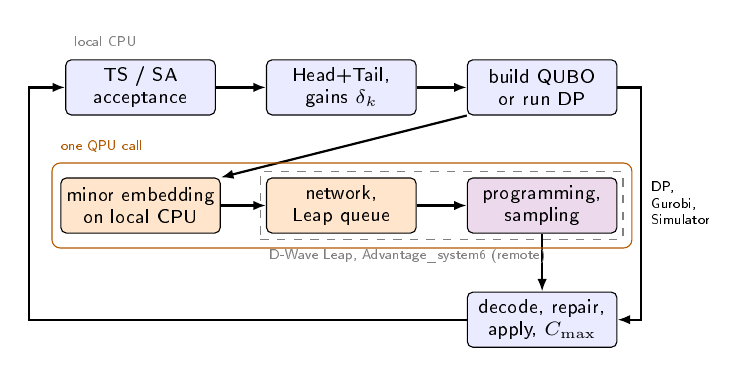
\begin{tikzpicture}[font=\sffamily\scriptsize,
  box/.style={draw,rounded corners=2pt,align=center,minimum height=7mm,minimum width=19mm,inner sep=2pt},
  arr/.style={-{Latex[length=1.6mm]},thick}]
\node[box,fill=blue!8] (meta) at (0,0) {TS / SA\\ acceptance};
\node[box,fill=blue!8] (eval) at (2.55,0) {Head+Tail,\\ gains $\delta_k$};
\node[box,fill=blue!8] (qubo) at (5.1,0) {build QUBO\\ or run DP};
\node[box,fill=orange!20] (emb) at (0,-1.5) {minor embedding\\ on local CPU};
\node[box,fill=orange!20] (net) at (2.55,-1.5) {network,\\ Leap queue};
\node[box,fill=violet!15] (qpu) at (5.1,-1.5) {programming,\\ sampling};
\node[box,fill=blue!8] (dec) at (5.1,-2.95) {decode, repair,\\ apply, $C_{\max}$};
\draw[arr] (meta)--(eval); \draw[arr] (eval)--(qubo);
\draw[arr] (qubo.south west)--(emb.north east);
\draw[arr] (emb)--(net); \draw[arr] (net)--(qpu);
\draw[arr] (qpu)--(dec);
\draw[arr] (qubo.east)--++(3mm,0)|-node[pos=0.25,right,font=\sffamily\tiny,align=left]{DP,\\ Gurobi,\\ Simulator}(dec.east);
\draw[arr] (dec.west)-|([xshift=-4mm]emb.west)|-(meta.west);
\node[draw,dashed,gray,fit=(net)(qpu),inner sep=2pt] (rem) {};
\node[gray,font=\sffamily\tiny,anchor=north west] at (rem.south west) {D-Wave Leap, Advantage\_system6 (remote)};
\node[draw,orange!70!black,rounded corners=3pt,fit=(emb)(net)(qpu)(rem),inner sep=3pt] (call) {};
\node[orange!70!black,font=\sffamily\tiny,anchor=south west] at (call.north west) {one QPU call};
\node[gray,font=\sffamily\tiny,anchor=south west] at ([yshift=1pt]meta.north west) {local CPU};
\end{tikzpicture}
\caption{\rev{Data flow in one iteration of the hybrid algorithm. The minor embedding is computed on the local CPU but belongs to the cost of one QPU call; with the dynamic program, Gurobi or the simulator the iteration stays on the local CPU.}}\label{fig:flow}
\end{figure}

\section{\rev{Neighborhood Structures}}\label{sec:neigh}
\begin{revblock}
All four neighborhoods are built from swaps. A swap $(i,j)$ with $i<j$ exchanges the jobs at positions $i$ and $j$, and the jobs between them stay in place (Fig.~\ref{fig:moves}a). The neighborhoods differ in which sets of swaps may be applied together. For a swap $(i,j)$ let $\delta_{ij}=C_{\max}(\pi')-C_{\max}(\pi)$ denote its gain, where $\pi'$ is $\pi$ after the swap, so a negative gain improves the schedule. We compute the gains with the Head+Tail technique~\cite{taillard1990some}. It combines the completion times of the unchanged prefix (heads) with the longest paths from the unchanged suffix to the end of the schedule (tails), so only the positions from $i$ to $j$ are recomputed, and one gain costs $O(m(j-i+1))$ time. The gain of a set of swaps is approximated by the sum of their gains. After the selection, the chosen swaps are applied and the makespan of the new permutation is computed from scratch with \eqref{eq:C11}--\eqref{eq:Ckj}. Every set allowed by one neighborhood is allowed by the next, so the neighborhoods form the chain Adjacent $\subset$ Fibonacci $\subset$ Dynasearch $\subset$ Motzkin. Counting the empty set, for $n$ positions they contain $n$, $F_{n+1}$, $2^{n-1}$ and $M_n$ move sets, where $F_k$ is the $k$-th Fibonacci number ($F_1=F_2=1$) and $M_n$ the $n$-th Motzkin number. For $n=20$ jobs the Adjacent neighborhood thus contains 20 move sets, the Fibonacci neighborhood 10\,946, the Dynasearch neighborhood 524\,288 and the Motzkin neighborhood more than 50 million, so the larger neighborhoods cannot be searched by listing their move sets one by one, and the best set has to be found by dynamic programming or through a QUBO model.
\end{revblock}

\subsection{\rev{Adjacent}}
\begin{revblock}
The Adjacent neighborhood contains the $n-1$ permutations obtained by one swap of neighboring positions $(i,i+1)$, $i=1,\dots,n-1$. With Head+Tail all $n-1$ gains $\delta_i=\delta_{i,i+1}$ cost $O(mn)$ time in total, and a scan finds the best swap in $O(n)$ time. The neighborhood changes the permutation only locally, and it is the baseline for the compound neighborhoods below.
\end{revblock}

\subsection{Fibonacci}
\begin{revblock}
The Fibonacci neighborhood~\cite{WojewodzkiBozejko2026} applies any set of adjacent swaps that do not overlap. If the swap $(i,i+1)$ is applied, the swaps $(i-1,i)$ and $(i+1,i+2)$ are not. Counting the empty set, there are $F_{n+1}$ such sets for $n$ positions. The best set is found by dynamic programming. Let $\delta_i$ be the gain of the swap $(i,i+1)$, and let $\mathcal{S}_i$ be the family of admissible sets that contain only swaps from $\{1,\dots,i\}$, including the empty set. For $i=0,\dots,n-1$ we define the value function
\begin{equation}\label{eq:fibV}
V(i)=\min_{S\in\mathcal{S}_i}\ \sum_{k\in S}\delta_k .
\end{equation}
$V(i)$ is the smallest total gain of an admissible set that changes only the first $i+1$ positions. The empty set has total gain $0$, so $V(i)\le 0$. The values of $V$ follow from the recurrence
\begin{align}
V(0)&=0, \quad V(1)=\min\{0,\,\delta_1\}, \label{eq:fib0}\\
V(i)&=\min\{V(i-1),\,V(i-2)+\delta_i\}, \nonumber\\
&\qquad i=2,\dots,n-1. \label{eq:fibrec}
\end{align}
The first term covers the sets without swap $i$. The second term covers the sets with swap $i$, which cannot contain swap $i-1$. The best set of the whole neighborhood has the total gain $V(n-1)$ and is recovered by tracing these choices back from $i=n-1$. This recurrence is the dynamic program of Dynasearch~\cite{Congram2002} restricted to adjacent swaps, and it takes $O(n)$ time after the $O(mn)$ evaluation of all gains. For TS the recurrence keeps the $\tau+1$ best sets in every state instead of one, which raises its cost to $O(n\tau)$. The empty set is not returned, so if no set improves the schedule, the best non-empty set is applied.
\end{revblock}

\begin{figure}[t]
\centering
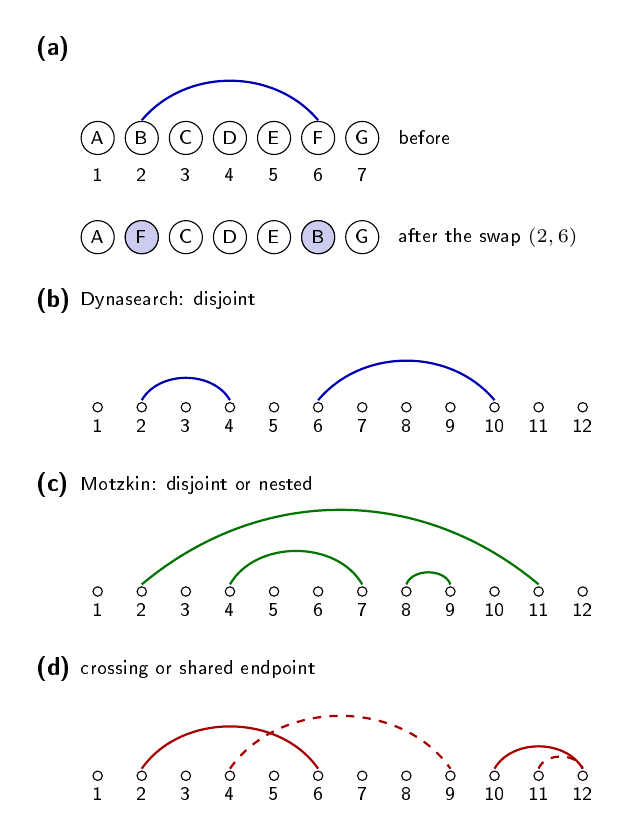
\begin{tikzpicture}[font=\sffamily\scriptsize,x=5.6mm,y=9mm]
% (a) jedna zamiana: przed i po
\node[anchor=west,font=\sffamily\small\bfseries] at (-0.6,1.25) {(a)};
\foreach \i/\j in {1/A,2/B,3/C,4/D,5/E,6/F,7/G} {
  \node[draw,circle,inner sep=1.2pt,minimum size=4.2mm,fill=white] at (\i,0) {\j};
  \node[below=2.5pt] at (\i,-0.2) {\i};
}
\draw[thick,blue!70!black] (2,0.25) to[bend left=50] (6,0.25);
\node[anchor=west] at (7.6,0) {before};
\foreach \i/\j in {1/A,2/F,3/C,4/D,5/E,6/B,7/G} {
  \node[draw,circle,inner sep=1.2pt,minimum size=4.2mm,fill=white] (q\i) at (\i,-1.4) {\j};
}
\node[draw,circle,inner sep=1.2pt,minimum size=4.2mm,fill=blue!70!black!20] at (2,-1.4) {F};
\node[draw,circle,inner sep=1.2pt,minimum size=4.2mm,fill=blue!70!black!20] at (6,-1.4) {B};
\node[anchor=west] at (7.6,-1.4) {after the swap $(2,6)$};
% (b)-(d)
\foreach \y/\lab/\nm in {-3.8/Dynasearch: disjoint/(b),-6.4/Motzkin: disjoint or nested/(c),-9.0/crossing or shared endpoint/(d)} {
  \node[anchor=west,font=\sffamily\small\bfseries] at (-0.6,\y+1.5) {\nm};
  \node[anchor=west,font=\sffamily\scriptsize] at (0.4,\y+1.5) {\lab};
  \foreach \i in {1,...,12} { \node[draw,circle,inner sep=1.2pt,fill=white] at (\i,\y) {}; \node[below=1pt] at (\i,\y) {\i}; }
}
\draw[thick,blue!70!black] (2,-3.7) to[bend left=60] (4,-3.7);
\draw[thick,blue!70!black] (6,-3.7) to[bend left=50] (10,-3.7);
\draw[thick,green!45!black] (2,-6.3) to[bend left=40] (11,-6.3);
\draw[thick,green!45!black] (4,-6.3) to[bend left=60] (7,-6.3);
\draw[thick,green!45!black] (8,-6.3) to[bend left=70] (9,-6.3);
\draw[thick,red!65!black] (2,-8.9) to[bend left=55] (6,-8.9);
\draw[thick,red!65!black,dashed] (4,-8.9) to[bend left=55] (9,-8.9);
\draw[thick,red!65!black] (10,-8.9) to[bend left=60] (12,-8.9);
\draw[thick,red!65!black,dashed] (11,-8.9) to[bend left=70] (12,-8.9);
\end{tikzpicture}
\caption{\rev{Swaps as arcs over job positions. (a)~The swap $(i,j)$ exchanges the jobs at positions $i$ and $j$ and leaves the jobs between them in place; (b)~Dynasearch allows only disjoint arcs, (c)~Motzkin also nested arcs, and (d)~crossing arcs and arcs with a shared endpoint are not allowed.}}\label{fig:moves}
\end{figure}

\subsection{\rev{Dynasearch}}
\begin{revblock}
The Dynasearch neighborhood~\cite{Congram2002} applies a set of swaps whose segments are pairwise disjoint (Fig.~\ref{fig:moves}b): the swaps $(i,j)$ and $(k,l)$ with $i<k$ can be applied together only if $j<k$. A segment may have any length, so there are $n(n-1)/2$ candidate swaps. One gain costs $O(m(j-i+1))$ time, and since $\sum_{i<j}(j-i+1)=O(n^3)$, all gains cost $O(mn^3)$. Let $D(j)$ be the smallest sum of gains over admissible sets inside positions $1,\dots,j$. Then
\begin{equation}
\begin{aligned}
D(0)&=0,\\
D(j)&=\min\Bigl\{D(j-1),\ \min_{1\le i<j}\bigl[D(i-1)+\delta_{ij}\bigr]\Bigr\},\\
&\qquad j=1,\dots,n.
\end{aligned}\label{eq:dyna}
\end{equation}
In this recurrence either no swap ends at position $j$, or the swap $(i,j)$ ends there and the swaps to the left of $i$ are chosen optimally. This recurrence takes $O(n^2)$ time, so the evaluation of the gains dominates, and one step of the neighborhood costs $O(mn^3)$. Counting the empty set, the neighborhood contains $2^{n-1}$ move sets. If no set improves the schedule, the single swap with the smallest gain is applied, so that the search always moves.
\end{revblock}

\subsection{\rev{Motzkin}}
\begin{revblock}
The Motzkin neighborhood~\cite{Motzkin_PWR_EXIT,Motzkin_PWR} also allows nested swaps. Two swaps $(i,j)$ and $(k,l)$ with $i<k$ can be applied together if their segments are disjoint ($j<k$) or nested ($l<j$), and they cannot if they cross ($k<j<l$) or share an endpoint (Fig.~\ref{fig:moves}c and~\ref{fig:moves}d). Swaps on four different positions exchange disjoint pairs of jobs, so they commute, and the result of a disjoint or nested set does not depend on the order of its swaps. Two swaps with a shared endpoint move three jobs along a cycle, and the result depends on the order, so such pairs are excluded. Crossing swaps would also commute, but they are excluded by the definition of the neighborhood. The non-crossing sets of swaps on $n$ positions correspond one-to-one to Motzkin paths of length $n$, which gives their number $M_n$~\cite{motzkin1948} and allows an exact interval dynamic program. Let $G(L,R)$ be the smallest sum of gains over admissible sets inside positions $L,\dots,R$, with $G(L,R)=0$ for $L\ge R$. Then
\begin{equation}
\begin{aligned}
G(L,R)=\min\Bigl\{&G(L+1,R),\\
&\min_{L<k\le R}\bigl[\delta_{Lk}+G(L+1,k-1)+G(k+1,R)\bigr]\Bigr\}.
\end{aligned}\label{eq:motz}
\end{equation}
In this recurrence either position $L$ is not swapped, or it is swapped with a position $k$, which splits the remaining positions into the inside $L+1,\dots,k-1$ and the outside $k+1,\dots,R$. The table has $O(n^2)$ entries, each computed in $O(n)$ time, so this recurrence runs in $O(n^3)$ time. With the $O(mn^3)$ evaluation of all $n(n-1)/2$ gains, one step of the Motzkin neighborhood costs $O(mn^3)$. As in Dynasearch, if no set improves the schedule, the single swap with the smallest gain is applied.
\end{revblock}

\begin{table}
\caption{\rev{Size and cost of the move selection for $n$ jobs and $m$ machines. $K$ is the number of QUBO variables and $|E|$ the number of nonzero quadratic coefficients; for Dynasearch and Motzkin both are upper bounds, reached when no candidate is removed, and the values in brackets are for $n=20$. DP is the cost of the dynamic program and $Q$ the cost of building the QUBO matrix.}}\label{tab:sizes}
\centering\footnotesize\ifrevmarks\color{red}\fi
\setlength{\tabcolsep}{3pt}
\begin{tabular}{@{}lccccc@{}}
\toprule
 & $K$ & gains $\delta_k$ & DP & $|E|$ & $Q$\\
\midrule
Adjacent   & $n-1$ & $O(mn)$ & $O(n)$ & $\binom{n-1}{2}$ & $O(n^2)$\\
           & (19) & & & (171; 100\%) & \\[2pt]
Fibonacci  & $n-1$ & $O(mn)$ & $O(n)$ & $n-2$ & $O(n)$\\
           & (19) & & & (18; 10.5\%) & \\[2pt]
Dynasearch & $\binom{n}{2}$ & $O(mn^3)$ & $O(n^2)$ & $\binom{K}{2}-\binom{n}{4}$ & $O(n^4)$\\
           & (190) & & & (13\,110; 73\%) & \\[2pt]
Motzkin    & $\binom{n}{2}$ & $O(mn^3)$ & $O(n^3)$ & $\binom{n}{4}+3\binom{n}{3}$ & $O(n^4)$\\
           & (190) & & & (8\,265; 46\%) & \\
\bottomrule
\end{tabular}

\smallskip\footnotesize\raggedright Applying the selected moves and computing the new makespan costs $O(mn)$ for every neighborhood. The table has no column for solving the QUBO model, because this cost depends on the solver (Section~\ref{sec:qubo}).
\end{table}

\section{\rev{QUBO Formulations of the Move Selection}}\label{sec:qubo}
\begin{revblock}
A QUBO model asks for a binary vector $\mathbf{x}\in\{0,1\}^K$ that minimizes
\begin{equation}
f(\mathbf{x})=\sum_{k=1}^{K}Q_{kk}x_k+\sum_{k<l}Q_{kl}x_kx_l=\mathbf{x}^\top Q\,\mathbf{x}
\end{equation}
\cite{Glover2019}. We use the upper-triangular convention of the \texttt{dimod} library: the linear coefficients lie on the diagonal of $Q$, every quadratic coefficient appears once, with $k<l$, and $Q_{kl}=0$ for $k>l$. Because $x_k^2=x_k$, every quadratic function of binary variables can be written in this form up to a constant. In our models the decision variable $x_k=1$ means that candidate move $k$ is selected, the linear coefficient carries the gain $\delta_k$ of this move, and the quadratic coefficients penalize pairs of moves that cannot be applied together. The substitution $x_k=(1+s_k)/2$ turns $f$ into the energy of an Ising model,
\begin{equation}
E(\mathbf{s})=\sum_k h_ks_k+\sum_{k<l}J_{kl}s_ks_l+\text{const},
\end{equation}
where $\mathbf{s}\in\{-1,1\}^K$, with $J_{kl}=Q_{kl}/4$ and $h_k=Q_{kk}/2+\sum_{l\ne k}Q_{\min(k,l),\max(k,l)}/4$. A quantum annealer realizes $E$ as its problem Hamiltonian~\cite{Kadowaki1998,Johnson2011}, so a low-energy spin state read from the processor corresponds to a binary vector with a low value of $f$. We use the word Hamiltonian only for this physical model and denote the QUBO objective by $f$. The QUBO model does not depend on the solver: it can be solved by classical algorithms, for example by simulated annealing, or sampled on a QPU, and Section~\ref{sec:setup} describes the solver used in our experiments.

All four models have the form $f(\mathbf{x})=\sum_k\delta_kx_k+P\cdot(\text{penalty})$, where the penalty is zero exactly for admissible selections. The following lemma gives a sufficient penalty weight.

\textbf{Lemma 1.} Let $E$ be the set of incompatible pairs of moves and $f(\mathbf{x})=\sum_k\delta_kx_k+P\sum_{(k,l)\in E}x_kx_l$. If $P>\max_k|\delta_k|$, every minimizer of $f$ selects a compatible set of moves, and the minimizers of $f$ are exactly the compatible sets with the smallest sum of gains. Likewise, if $P>\max_k|\delta_k|$, every minimizer of $g(\mathbf{x})=\sum_k\delta_kx_k+P\bigl(\sum_kx_k-1\bigr)^2$ selects exactly one move.

\emph{Proof.} Let $\mathbf{x}$ select an incompatible pair, and let $k$ be a selected move of this pair. Setting $x_k=0$ changes $f$ by $-\delta_k-P\,d_k$, where $d_k\ge 1$ is the number of selected moves incompatible with $k$, so the change is at most $|\delta_k|-P<0$ and $\mathbf{x}$ is not a minimizer. On compatible selections $f$ equals the sum of gains, which proves the first claim. For $g$, the zero vector has the value $P>\min_k\delta_k$, the value of the best one-hot vector. If $\mathbf{x}$ selects $s\ge 2$ moves, dropping a selected move $k$ changes $g$ by $-\delta_k-P(2s-3)\le|\delta_k|-P<0$. $\square$

Any weight above this bound gives the same minimizers, so $P$ does not change the model, but it changes its numerical scale. The QPU accepts coefficients only in a bounded range, and the sampler rescales the whole model to fit it. A large $P$ therefore compresses the differences between the gains into a small part of the range, where they compete with the analog control errors of the device~\cite{dwave_handbook}. For classical samplers a large $P$ makes every step out of a feasible state expensive, which slows the search down~\cite{Glover2019}. The weights used in our experiments, $P=2\max_i|\delta_i|+1$ for the Adjacent model and $P=\sum_k|\delta_k|+1$ for the other models, satisfy Lemma~1, but the second one is up to $K$ times larger than necessary.
\end{revblock}

\subsection{\rev{QUBO formulation of the Adjacent selection}}
\begin{revblock}
The Adjacent selection chooses one swap of neighboring positions. The variable $x_i=1$ selects the swap $(i,i+1)$, $i=1,\dots,n-1$, with the gain $\delta_i$, and the model
\begin{equation}
g(\mathbf{x})=\sum_{i=1}^{n-1}\delta_ix_i+P\Bigl(\sum_{i=1}^{n-1}x_i-1\Bigr)^2
\end{equation}
selects exactly one swap when $P>\max_i|\delta_i|$ (Lemma~1); we used $P=2\max_i|\delta_i|+1$. Expanding the square with $x_i^2=x_i$ gives $Q_{ii}=\delta_i-P$ and $Q_{ij}=2P$ for $i<j$, plus the constant $P$. Every pair of variables is coupled, so the graph of the model is complete, with $(n-1)(n-2)/2$ quadratic coefficients (171 for $n=20$). Building $Q$ takes $O(n^2)$ time after the $O(mn)$ evaluation of the gains, and applying the selected swap and computing the new makespan takes $O(mn)$ time. The cost of solving the model depends on the solver. A scan finds the best swap in $O(n)$ time, so this model measures the cost of a QPU call rather than offering a faster selection.
\end{revblock}

\subsection{\rev{QUBO formulation of the Fibonacci selection}}
\begin{revblock}
The variables are those of the Adjacent model, but any set of non-overlapping swaps may be selected. The swaps $i$ and $i+1$ share position $i+1$, so every such pair is penalized:
\begin{equation}
f(\mathbf{x})=\sum_{i=1}^{n-1}\delta_ix_i+P\sum_{i=1}^{n-2}x_ix_{i+1}.
\end{equation}
In the upper-triangular convention $Q$ has the gains on its diagonal and $P$ on its first superdiagonal, so it is bidiagonal, and the graph of the model is a path with $n-2$ edges (18 for $n=20$, about 10\% of all pairs). By Lemma~1 the minimizers of $f$ are the optimal sets found by the dynamic program \eqref{eq:fibV}--\eqref{eq:fibrec}. We used $P=\sum_i|\delta_i|+1$, which satisfies the lemma. All $n-1$ candidates enter the model, and building $Q$ takes $O(n)$ time.
\end{revblock}

\subsection{\rev{QUBO formulation of the Dynasearch selection}}
\begin{revblock}
We write the Dynasearch selection, the choice of a set of swaps with disjoint segments, as a QUBO model. The variable $x_k=1$ selects the swap of the endpoints of the segment $[i_k,j_k]$, with the gain $\delta_k$. Two swaps overlap if $\max(i_k,i_l)\le\min(j_k,j_l)$, which covers crossing and nested segments and segments with a shared endpoint, and every overlapping pair is penalized:
\begin{equation}
f(\mathbf{x})=\sum_k\delta_kx_k+P\sum_{k<l,\ \mathrm{overlap}(k,l)}x_kx_l.
\end{equation}
Before the model is built, candidates with $\delta_k\ge 0$ are removed. This does not change the optimum, because dropping such a move from a compatible set keeps the set compatible and does not increase its sum of gains. Without the filter the model has $K=n(n-1)/2$ variables, and since only the $\binom{n}{4}$ disjoint pairs are compatible, it has $\binom{K}{2}-\binom{n}{4}$ quadratic coefficients. For $n=20$ this gives 190 variables and 13\,110 of the 17\,955 pairs (73\%), and the share of coupled pairs tends to $2/3$ as $n$ grows, so the model is dense. The filter reduces these numbers by an amount that depends on the instance and on the current permutation. We used $P=\sum_k|\delta_k|+1$ over the remaining candidates. Building $Q$ takes $O(K^2)=O(n^4)$ time after the $O(mn^3)$ evaluation of the gains.
\end{revblock}

\subsection{\rev{QUBO formulation of the Motzkin selection}}
\begin{revblock}
The variables are the endpoint swaps of the Dynasearch model, again without candidates with $\delta_k\ge 0$. Two swaps $k$ and $l$ are incompatible if they share an endpoint, $\{i_k,j_k\}\cap\{i_l,j_l\}\ne\emptyset$, or if they cross, $i_k<i_l<j_k<j_l$ or $i_l<i_k<j_l<j_k$; disjoint and nested pairs are compatible. The model
\begin{equation}
f(\mathbf{x})=\sum_k\delta_kx_k+P\sum_{k<l,\ \mathrm{conflict}(k,l)}x_kx_l
\end{equation}
has $\delta_k$ on the diagonal of $Q$ and $P$ at the positions of incompatible pairs. Without the filter there are $\binom{n}{4}$ crossing pairs and $3\binom{n}{3}$ pairs with a shared endpoint, which for $n=20$ gives at most 8\,265 of the 17\,955 pairs (46\%); the share tends to $1/3$ as $n$ grows. We used $P=\sum_k|\delta_k|+1$. Building $Q$ takes $O(K^2)=O(n^4)$ time after the $O(mn^3)$ evaluation of the gains.
\end{revblock}

\section{\rev{Experimental Setup}}\label{sec:setup}
\begin{revblock}
\paragraph{Hardware and software.} The metaheuristics, the evaluation of the gains, the dynamic programs, the construction of the QUBO models, Gurobi and the simulator ran on a MacBook Pro with an Apple M4 Pro processor and 24~GB of RAM, under macOS 26.3.1 and Python 3.11. The QUBO models were built with the \texttt{dimod} library. The experiments with the dynamic programs, Gurobi and the simulator ran on 8 November 2026, and the experiments on the QPU on 9 November 2026.

\paragraph{Solvers.} The move is selected in four ways, shown as the four groups of rows in Tables~\ref{tab:results_ts} and~\ref{tab:results_sa}. In the rows ``Classical DP'' the dynamic programs of Section~\ref{sec:neigh} select the move, and for the Adjacent neighborhood a scan of all swaps does. In the other rows the QUBO model of Section~\ref{sec:qubo} is built and solved. In the rows ``Gurobi'', Gurobi 13.0.3 solved it exactly, with one thread and a zero optimality gap, so every call returned a minimizer of the model. In the rows ``Simulator'', it was solved by \texttt{SimulatedAnnealingSampler} of the \texttt{dwave-samplers} library (version 1.7.0, part of the Ocean SDK), a classical simulated annealing heuristic in C++ that runs on the CPU and does not simulate quantum hardware. Every call performed 1000 reads, each starting from a random state and making 1000 sweeps of single-variable Metropolis updates with a geometric schedule of the inverse temperature, whose range the library sets from the coefficients of the model. The seed of every call was drawn from the random number generator of the run. In the rows ``QPU'', the models were sampled on the D-Wave Advantage\_system6 quantum annealer, with the Pegasus topology, through the Leap cloud service, with the \texttt{DWaveSampler} of the Ocean SDK (\texttt{dwave-system} 1.34.0). All results in the rows ``QPU'' come from runs on this physical processor, and no part of them was simulated. A new connection to the service was opened at every call. Every model sent to the QPU was passed to an \texttt{EmbeddingComposite}, which computes a minor embedding with the \texttt{minorminer} heuristic~\cite{Cai2014} at every call and does not reuse it. Every QPU call requested 1000 samples, and the annealing time, the chain strength and the spin-reversal setting were left at the default values of the solver and of the Ocean SDK. The solution returned by Gurobi and the sample with the lowest energy returned by the simulator or the QPU were decoded into a set of moves, and moves that conflict with each other were removed greedily, so the applied set was always admissible. If the decoded set was empty, the Adjacent variant applied the swap with the smallest gain, and the other variants applied it only if its gain was negative; otherwise the permutation did not change. For every QPU call we recorded the time of the connection, the time of finding the embedding, the QPU access time reported by the solver and the total wall-clock time of the call, and Section~\ref{sec:results} reports these components.

\paragraph{Instances and runs.} We used the first 30 Taillard instances~\cite{ref_taillard}, ten for each size with $n=20$ and $m\in\{5,10,20\}$. Every combination of metaheuristic, neighborhood and solver was run once on each instance, with the random seed 0 and the budget $t_{\max}=10\,000$~ms. The results for the shorter budgets $t_{\max}\in\{100,500,1000,2000,5000\}$~ms were read from the same run: at the start of the first iteration at which the elapsed time had reached a budget, we stored the best permutation found so far. The budget is checked only before an iteration, so this is exactly the result of a run with the shorter budget that makes the same random choices. TS used the tabu tenure $\tau=10$. SA used $T_{\text{init}}=1000$, $T_{\text{final}}=1$ and $\alpha=0.95$, so its temperature reaches $T_{\text{final}}$ after 135 iterations, and reheating with $r=1.5$ and $t_{\text{stag}}=500$~ms. The segments of Dynasearch and Motzkin were not limited in length. These values were set in advance and not tuned.

\paragraph{Metric.} Each table entry is the mean relative percentage deviation $\mathrm{RPD}=100\%\cdot(C_{\max}-LB)/LB$ over the ten instances of one size, where $LB$ is the lower bound published for the instance by Taillard~\cite{ref_taillard}. The lower bound is below the best known makespan, so RPD overstates the distance to the best known solutions, but it is the same reference for all variants. Convergence is shown as $C_{\max}$ against wall-clock time.
\end{revblock}

\begin{table*}
\caption{\rev{Mean RPD~[\%] from the lower bound for TS by solver, neighborhood, budget $t_{\max}$ and number of machines ($n=20$)}}
\label{tab:results_ts}
\centering\scriptsize\ifrevmarks\color{red}\fi
\setlength{\tabcolsep}{2.4pt}
\begin{tabular}{@{}ll rrrr rrrr rrrr rrrr rrrr rrrr@{}}
& & \multicolumn{4}{c}{100~ms} & \multicolumn{4}{c}{500~ms} & \multicolumn{4}{c}{1\,000~ms} & \multicolumn{4}{c}{2\,000~ms} & \multicolumn{4}{c}{5\,000~ms} & \multicolumn{4}{c}{10\,000~ms} \\
\cmidrule(lr){3-6}\cmidrule(lr){7-10}\cmidrule(lr){11-14}\cmidrule(lr){15-18}\cmidrule(lr){19-22}\cmidrule(lr){23-26}
\textbf{Solver} & \textbf{Neigh.} & 5 & 10 & 20 & AVG & 5 & 10 & 20 & AVG & 5 & 10 & 20 & AVG & 5 & 10 & 20 & AVG & 5 & 10 & 20 & AVG & 5 & 10 & 20 & AVG \\
\hline
\multirow{4}{*}{Classical DP} & adj & 5.81 & 15.74 & 28.44 & 16.66 & 4.44 & 12.92 & 24.91 & 14.09 & 4.26 & 12.60 & 23.60 & 13.49 & 4.17 & 12.47 & 22.35 & 13.00 & 3.99 & 11.83 & 21.86 & 12.56 & 3.90 & 11.73 & 21.75 & 12.46 \\
 & fib & 18.04 & 25.61 & 34.42 & 26.02 & 18.04 & 25.61 & 34.42 & 26.02 & 18.04 & 25.61 & 34.42 & 26.02 & 18.04 & 25.61 & 34.42 & 26.02 & 18.04 & 25.61 & 34.42 & 26.02 & 18.04 & 25.61 & 34.42 & 26.02 \\
 & dyn & \textbf{4.04} & \textbf{12.37} & \textbf{24.20} & \textbf{13.54} & \textbf{3.48} & 11.46 & \textbf{22.64} & \textbf{12.53} & \textbf{3.07} & \textbf{11.27} & \textbf{22.27} & \textbf{12.20} & \textbf{2.93} & 11.07 & 22.12 & \textbf{12.04} & \textbf{2.87} & 10.72 & 21.83 & 11.81 & \textbf{2.64} & 10.31 & \textbf{21.64} & \textbf{11.53} \\
 & mot & 4.66 & 13.40 & 24.29 & 14.12 & 3.58 & \textbf{11.32} & 23.05 & 12.65 & 3.31 & 11.28 & 22.33 & 12.31 & 3.23 & \textbf{11.06} & \textbf{22.06} & 12.12 & 3.05 & \textbf{10.57} & \textbf{21.69} & \textbf{11.77} & 2.89 & \textbf{10.29} & 21.67 & 11.62 \\
\hline
\multirow{4}{*}{Gurobi} & adj & 20.59 & 33.42 & 40.31 & 31.44 & 16.09 & 27.24 & 35.16 & 26.16 & 14.75 & 25.15 & 33.90 & 24.60 & 12.28 & 23.61 & 32.23 & 22.71 & 11.29 & 22.02 & 31.03 & 21.45 & 10.09 & 20.35 & 30.38 & 20.27 \\
 & fib & 10.79 & 21.49 & 30.77 & 21.02 & 8.16 & 17.90 & 28.51 & 18.19 & 7.34 & 17.13 & 27.99 & 17.49 & 6.97 & 16.59 & 27.12 & 16.89 & 5.89 & 16.16 & 25.97 & 16.01 & 5.82 & 15.78 & 25.80 & 15.80 \\
 & dyn & 13.52 & 18.14 & 29.73 & 20.46 & 5.39 & 12.75 & 23.51 & 13.88 & 4.57 & 12.14 & 23.17 & 13.29 & 3.96 & 11.28 & 23.03 & 12.76 & 3.51 & 11.00 & 22.76 & 12.42 & 3.25 & 10.98 & 22.33 & 12.19 \\
 & mot & 15.48 & 26.86 & 34.23 & 25.52 & 9.26 & 18.81 & 27.23 & 18.43 & 6.33 & 16.11 & 24.73 & 15.72 & 4.96 & 13.70 & 23.62 & 14.09 & 4.23 & 12.23 & 22.55 & 13.00 & 4.01 & 11.51 & 22.07 & 12.53 \\
\hline
\multirow{4}{*}{Simulator} & adj & 24.98 & 37.47 & 43.89 & 35.45 & 22.11 & 34.79 & 41.26 & 32.72 & 19.72 & 33.24 & 39.70 & 30.89 & 18.26 & 31.35 & 37.94 & 29.18 & 15.22 & 26.71 & 35.08 & 25.67 & 12.27 & 25.24 & 33.30 & 23.60 \\
 & fib & 23.57 & 35.40 & 42.01 & 33.66 & 17.35 & 30.16 & 38.37 & 28.63 & 15.76 & 27.89 & 36.38 & 26.68 & 14.53 & 26.62 & 35.63 & 25.59 & 13.39 & 23.73 & 33.82 & 23.65 & 12.07 & 23.23 & 31.43 & 22.24 \\
 & dyn & 18.17 & 29.68 & 38.33 & 28.73 & 17.42 & 29.68 & 38.33 & 28.48 & 15.01 & 29.16 & 37.27 & 27.15 & 11.11 & 23.18 & 34.19 & 22.83 & 5.95 & 14.90 & 26.40 & 15.75 & 4.39 & 13.45 & 24.88 & 14.24 \\
 & mot & 19.83 & 32.71 & 38.84 & 30.46 & 18.87 & 32.71 & 38.84 & 30.14 & 17.76 & 32.22 & 38.14 & 29.37 & 14.86 & 27.27 & 35.62 & 25.92 & 11.17 & 19.32 & 31.12 & 20.54 & 10.52 & 16.97 & 27.43 & 18.31 \\
\hline
\multirow{4}{*}{QPU} & adj & 24.98 & 37.47 & 43.89 & 35.45 & 24.98 & 37.47 & 43.89 & 35.45 & 24.98 & 37.47 & 43.89 & 35.45 & 24.05 & 37.11 & 42.73 & 34.63 & 22.36 & 35.34 & 41.26 & 32.99 & 19.75 & 33.13 & 39.60 & 30.83 \\
 & fib & 23.19 & 35.08 & 42.35 & 33.54 & 23.19 & 35.08 & 42.35 & 33.54 & 23.19 & 35.08 & 42.35 & 33.54 & 22.19 & 33.21 & 40.01 & 31.80 & 19.68 & 32.40 & 38.23 & 30.10 & 16.69 & 30.45 & 36.73 & 27.96 \\
 & dyn & 24.03 & 37.21 & 42.57 & 34.60 & 24.03 & 37.21 & 42.57 & 34.60 & 24.03 & 37.21 & 42.57 & 34.60 & 24.03 & 37.21 & 42.57 & 34.60 & 23.16 & 37.21 & 42.57 & 34.31 & 22.05 & 36.95 & 42.23 & 33.74 \\
 & mot & 20.34 & 33.39 & 40.65 & 31.46 & 20.34 & 33.39 & 40.65 & 31.46 & 20.34 & 33.39 & 40.65 & 31.46 & 20.34 & 33.39 & 40.65 & 31.46 & 18.86 & 33.39 & 40.65 & 30.97 & 17.60 & 32.24 & 40.06 & 29.97 \\
\hline
\end{tabular}


\vspace{3mm}
\caption{\rev{Mean RPD~[\%] from the lower bound for SA by solver, neighborhood, budget $t_{\max}$ and number of machines ($n=20$)}}
\label{tab:results_sa}
\setlength{\tabcolsep}{1.4pt}
\begin{tabular}{@{}ll rrrr rrrr rrrr rrrr rrrr rrrr@{}}
& & \multicolumn{4}{c}{100~ms} & \multicolumn{4}{c}{500~ms} & \multicolumn{4}{c}{1\,000~ms} & \multicolumn{4}{c}{2\,000~ms} & \multicolumn{4}{c}{5\,000~ms} & \multicolumn{4}{c}{10\,000~ms} \\
\cmidrule(lr){3-6}\cmidrule(lr){7-10}\cmidrule(lr){11-14}\cmidrule(lr){15-18}\cmidrule(lr){19-22}\cmidrule(lr){23-26}
\textbf{Solver} & \textbf{Neigh.} & 5 & 10 & 20 & AVG & 5 & 10 & 20 & AVG & 5 & 10 & 20 & AVG & 5 & 10 & 20 & AVG & 5 & 10 & 20 & AVG & 5 & 10 & 20 & AVG \\
\hline
\multirow{4}{*}{Classical DP} & adj & 17.24 & 31.02 & 38.05 & 28.77 & 17.24 & 31.02 & 38.05 & 28.77 & 17.24 & 31.02 & 38.05 & 28.77 & 17.24 & 31.02 & 38.05 & 28.77 & 17.24 & 31.02 & 38.05 & 28.77 & 17.24 & 31.02 & 38.05 & 28.77 \\
 & fib & 18.42 & 30.22 & 36.88 & 28.51 & 18.42 & 30.22 & 36.88 & 28.51 & 18.42 & 30.22 & 36.88 & 28.51 & 18.42 & 30.22 & 36.88 & 28.51 & 18.42 & 30.22 & 36.88 & 28.51 & 18.42 & 30.22 & 36.88 & 28.51 \\
 & dyn & \textbf{6.18} & \textbf{14.68} & \textbf{24.83} & \textbf{15.23} & \textbf{6.18} & \textbf{14.68} & 24.83 & \textbf{15.23} & \textbf{6.18} & \textbf{14.68} & 24.83 & \textbf{15.23} & \textbf{6.18} & \textbf{14.68} & 24.83 & \textbf{15.23} & \textbf{6.18} & \textbf{14.68} & 24.83 & \textbf{15.23} & \textbf{6.18} & \textbf{14.68} & 24.83 & \textbf{15.23} \\
 & mot & 8.39 & 17.61 & 25.69 & 17.23 & 8.39 & 17.61 & 25.49 & 17.16 & 8.39 & 17.61 & 25.49 & 17.16 & 8.39 & 17.61 & 25.49 & 17.16 & 8.39 & 17.61 & 25.49 & 17.16 & 8.39 & 17.61 & 25.49 & 17.16 \\
\hline
\multirow{4}{*}{Gurobi} & adj & 20.22 & 33.66 & 40.14 & 31.34 & 17.57 & 31.33 & 38.30 & 29.07 & 17.57 & 31.33 & 38.30 & 29.07 & 17.57 & 31.33 & 38.30 & 29.07 & 17.57 & 31.33 & 38.30 & 29.07 & 17.57 & 31.33 & 38.30 & 29.07 \\
 & fib & 18.42 & 29.80 & 36.88 & 28.37 & 18.42 & 29.80 & 36.88 & 28.37 & 18.42 & 29.80 & 36.88 & 28.37 & 18.42 & 29.80 & 36.88 & 28.37 & 18.42 & 29.80 & 36.88 & 28.37 & 18.42 & 29.80 & 36.88 & 28.37 \\
 & dyn & 13.52 & 17.71 & 29.80 & 20.34 & 7.26 & 15.68 & \textbf{24.34} & 15.76 & 7.26 & 15.68 & \textbf{24.34} & 15.76 & 7.26 & 15.68 & \textbf{24.34} & 15.76 & 7.26 & 15.68 & \textbf{24.34} & 15.76 & 7.26 & 15.68 & \textbf{24.34} & 15.76 \\
 & mot & 15.48 & 26.86 & 34.23 & 25.52 & 10.49 & 19.61 & 28.79 & 19.63 & 9.74 & 18.92 & 27.35 & 18.67 & 9.74 & 18.53 & 27.07 & 18.45 & 9.74 & 18.53 & 27.07 & 18.45 & 9.74 & 18.53 & 27.07 & 18.45 \\
\hline
\multirow{4}{*}{Simulator} & adj & 24.98 & 37.47 & 43.89 & 35.45 & 21.87 & 34.79 & 41.41 & 32.69 & 19.72 & 33.20 & 39.70 & 30.87 & 18.07 & 31.18 & 37.65 & 28.97 & 15.57 & 28.98 & 36.43 & 26.99 & 14.89 & 27.65 & 36.18 & 26.24 \\
 & fib & 23.57 & 35.40 & 42.01 & 33.66 & 17.35 & 30.73 & 38.37 & 28.82 & 16.28 & 28.07 & 36.34 & 26.90 & 14.67 & 27.17 & 35.59 & 25.81 & 13.80 & 26.09 & 34.75 & 24.88 & 13.09 & 25.81 & 34.38 & 24.43 \\
 & dyn & 18.17 & 29.68 & 38.33 & 28.73 & 17.42 & 29.68 & 38.33 & 28.48 & 15.01 & 29.16 & 37.27 & 27.15 & 11.11 & 23.18 & 34.19 & 22.83 & 6.65 & 15.13 & 26.18 & 15.99 & 6.65 & 15.13 & 25.73 & 15.84 \\
 & mot & 19.83 & 32.71 & 38.84 & 30.46 & 18.87 & 32.71 & 38.84 & 30.14 & 17.67 & 32.22 & 38.14 & 29.34 & 15.02 & 27.68 & 35.19 & 25.96 & 10.91 & 21.74 & 29.24 & 20.63 & 8.43 & 17.38 & 27.96 & 17.92 \\
\hline
\multirow{4}{*}{QPU} & adj & 24.98 & 37.47 & 43.89 & 35.45 & 24.98 & 37.47 & 43.89 & 35.45 & 24.98 & 37.47 & 43.89 & 35.45 & 23.87 & 37.08 & 42.97 & 34.64 & 22.13 & 34.87 & 41.26 & 32.75 & 20.42 & 33.21 & 39.56 & 31.06 \\
 & fib & 23.43 & 35.76 & 42.36 & 33.85 & 23.43 & 35.76 & 42.36 & 33.85 & 23.43 & 35.76 & 42.36 & 33.85 & 21.34 & 33.95 & 39.71 & 31.67 & 19.65 & 32.02 & 37.98 & 29.88 & 17.20 & 30.25 & 35.91 & 27.79 \\
 & dyn & 22.07 & 36.59 & 42.95 & 33.87 & 22.07 & 36.59 & 42.95 & 33.87 & 22.07 & 36.59 & 42.95 & 33.87 & 22.07 & 36.59 & 42.95 & 33.87 & 21.56 & 36.59 & 42.54 & 33.56 & 20.38 & 35.60 & 42.02 & 32.67 \\
 & mot & 21.24 & 35.76 & 41.12 & 32.71 & 21.24 & 35.76 & 41.12 & 32.71 & 21.24 & 35.76 & 41.12 & 32.71 & 21.24 & 35.76 & 41.12 & 32.71 & 20.32 & 35.76 & 41.12 & 32.40 & 18.31 & 34.91 & 40.14 & 31.12 \\
\hline
\end{tabular}

\end{table*}


\section{\rev{Results and Discussion}}\label{sec:results}
\begin{revblock}
Tables~\ref{tab:results_ts} and~\ref{tab:results_sa} give the mean RPD of every variant for the six budgets.

\paragraph{Classical DP.} Dynasearch and Motzkin give the best schedules for every budget and every instance size, in both metaheuristics, and TS is better than SA for every neighborhood. One DP selection in these neighborhoods costs $O(mn^3)$ time, but one step improves the schedule much more than an adjacent swap. TS with the Fibonacci neighborhood gives the same result for every budget. The tabu list forbids only the repetition of the same set of swaps, and the search cycles among a few permutations reached by different sets.

\paragraph{Simulated annealing.} The RPD of every SA variant with DP selection is the same for all six budgets. The results for all budgets come from one run, so SA found its best solution within the first 100~ms and did not improve it later. SA starts from the identity permutation and applies the best move of the neighborhood, so it descends to the first local optimum. There the best move worsens the schedule. When the Metropolis rule accepts it, the reverse move improves the schedule by the same amount, and the search returns to the same local optimum. The temperature reaches $T_{\text{final}}$ within 135 iterations. Reheating multiplies it by $r=1.5$ after 500~ms without improvement, but the following iterations lower it back to $T_{\text{final}}$ within eight steps, so in our runs reheating had no visible effect. Figure~\ref{fig:conv_sa_tai20_20} shows that with the DP selection the SA curves become flat within the first hundred milliseconds, while the simulator and the QPU still improve the schedule after several seconds.
\end{revblock}

\begin{figure}
\begin{center}
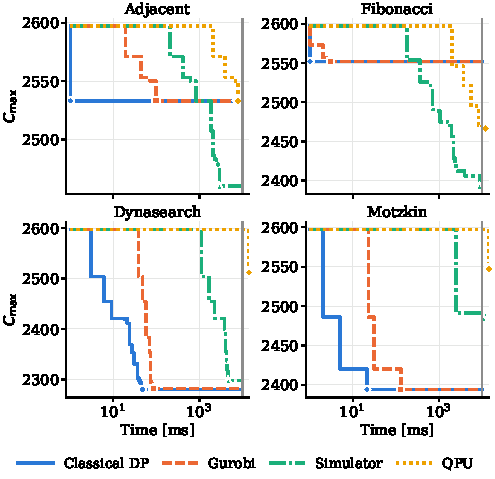
\includegraphics[width=0.99\linewidth]{img/conv_sa_tai20_20_inst5.pdf}
\end{center}
\caption{\rev{Best makespan found by SA on instance tai026 ($n=20$, $m=20$) with the four solvers. The vertical line marks $t_{\max}=10\,000$~ms.}}
\label{fig:conv_sa_tai20_20}
\end{figure}

\begin{revblock}
\paragraph{QUBO models solved classically.} The variants that solve the QUBO models on a classical computer separate the effect of the model from the effect of the processor. Lemma~1 in Section~\ref{sec:qubo} shows that the best solution of every model is exactly the move set chosen by the dynamic program, and in our tests Gurobi returned move sets with the same sum of gains as the dynamic program, so the model itself loses nothing. The cost lies in solving it. One call of Gurobi takes from below 1~ms for the Fibonacci model to about 25~ms for the Adjacent model, and one call of the simulator with 1000 reads takes 0.2 to 0.65~s, while the dynamic program needs at most a few milliseconds. With Gurobi, TS with the Dynasearch and Motzkin neighborhoods comes within one percentage point of the DP selection at $t_{\max}=10\,000$~ms, and with the simulator it stays further behind.

In TS the QUBO variants also handle tabu moves differently. They return a single move and restart from a random permutation when this move is tabu, whereas the Adjacent and Fibonacci procedures with DP selection take the best non-tabu move among their $\tau+1$ best moves. For the Fibonacci neighborhood the restarts break the cycle described above, and Gurobi and the simulator both give better schedules than the DP selection. In SA the simulator gives better schedules than the DP selection for the Adjacent and Fibonacci neighborhoods, most likely because its suboptimal samples act as random perturbations that move the search away from the local optimum. In most SA runs with the Dynasearch model and in some with the Motzkin model the simulator is no longer called after the search reaches a local optimum, because no candidate with a negative gain is left and the model is empty.

\paragraph{QPU.} In every variant except SA with the Fibonacci neighborhood, where the DP selection itself stagnates, the real QPU, Advantage\_system6, gives the worst schedules at $t_{\max}=10\,000$~ms. The processor takes little of this time. The median QPU access time of one call, which covers programming the processor and 1000 reads, is 0.11 to 0.16~s, while the whole call takes about 2~s for the Adjacent and Fibonacci models and 8 to 11~s for the Dynasearch and Motzkin models. Most of the remaining time goes to finding the minor embedding on the local CPU, 5 to 8~s in the median for the dense models, and to the network and the queue of the Leap service, 1.5 to 2.3~s. Within the budget TS and SA therefore perform 5 or 6 calls with the Adjacent and Fibonacci models and a single call with the Dynasearch and Motzkin models, against thousands of iterations with the DP selection. Figure~\ref{fig:conv_ils_tai20_5} shows this for TS on one instance: with the DP selection the curves fall within the first second, while the QPU variants of Dynasearch and Motzkin change the schedule once, at the end of the run. The samples of the dense models are also less accurate. For the Adjacent and Fibonacci models the lowest-energy sample was an optimum of the model in more than 99\% of the calls, but for the Dynasearch and Motzkin models only in about a quarter of the calls, and in 62\% and 36\% of the calls it violated the constraints, so the greedy repair had to remove moves.
\end{revblock}

\begin{figure}
\begin{center}
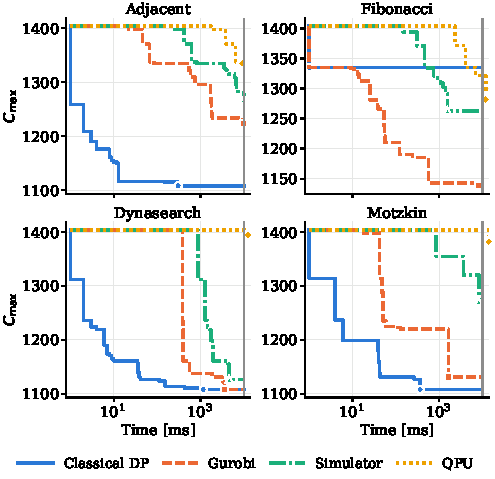
\includegraphics[width=0.99\linewidth]{img/conv_ils_tai20_5_inst9.pdf}
\end{center}
\caption{\rev{Best makespan found by TS on instance tai010 ($n=20$, $m=5$) with the four solvers. The vertical line marks $t_{\max}=10\,000$~ms.}}
\label{fig:conv_ils_tai20_5}
\end{figure}

\begin{revblock}
\paragraph{Limitations.} The experiments were conducted only on instances with $n=20$. The size of the instances is limited by minor embedding rather than by the number of qubits alone. For $n=20$ the Adjacent and Fibonacci models have 19 variables, and the Dynasearch and Motzkin models up to 190 variables with up to 13\,110 and 8\,265 quadratic coefficients (Table~\ref{tab:sizes}). A dense model has to be embedded as a clique minor, in which every variable occupies a chain of physical qubits, and the chains grow with the number of variables~\cite{Cai2014}. In our runs the embedded Dynasearch and Motzkin models occupied up to 1991 and 1870 physical qubits, with chains of up to 30 and 22 qubits. Already for $n=50$ the unfiltered Dynasearch model would have 1\,225 variables and 519\,400 quadratic coefficients. In a test on the local CPU, the Dynasearch and Motzkin models for $n=50$ could not be embedded into the Advantage processor, which does not have enough qubits for the chains that these dense models need. A precomputed clique embedding, reused in every call, would remove most of the embedding time for the dense models. The SA parameters were set in advance and not tuned, and the results above show that they let SA stagnate. Larger instances need a decomposition of the models, which a separate study addresses~\cite{WojewodzkiBozejkoSSRN}.
\end{revblock}

%%%%%%%%%%%%%%%%%%%%%%%%%%%%%%%%%%%%%%%%%%%%%%%%%%%%%%%
%% ACKNOWLEDGEMENTS
% \begin{acknowledgements}
% Avoid the stilted expression “one of us (R. B. G.) thanks ...”.  Instead, try “R. B. G. thanks...”. Put sponsor acknowledgements unnumbered at the end of the text and before References.
% \end{acknowledgements}
%%%%%%%%%%%%%%%%%%%%%%%%%%%%%%%%%%%%%%%%%%%%%%%%%%%%%%%
%% REFERENCES
%% Since January 1st 2021, IEEE Citation Style should be applied.
%\bibliographystyle{IEEEtran}


\section*{Declaration of Generative AI Use}
Generative AI and AI-assisted technologies were used in the preparation of this manuscript solely to improve readability and language. The scientific content, analysis, results, and conclusions were developed entirely by the authors. All AI-assisted outputs were carefully reviewed and edited by the authors, who take full responsibility for the content of the manuscript.


\bibliographystyle{IEEEtranUrldate}

%% Change to your *.bst file
\bibliography{sampleBibFile}

\end{document}


